\documentclass[12pt,a4paper]{article}

\usepackage[T1]{fontenc}
\usepackage[utf8]{inputenc}
\usepackage[polish]{babel}
\usepackage{lmodern}
\usepackage[a4paper,margin=2.5cm]{geometry}
\usepackage{amsmath,amssymb}
\usepackage{graphicx}
\usepackage{booktabs}
\usepackage{array}
\usepackage{float}
\usepackage{caption}
\usepackage{enumitem}
\usepackage{xcolor}
\usepackage{listings}
\usepackage{tikz}
\usetikzlibrary{shapes.geometric,arrows.meta}
\usepackage[hidelinks]{hyperref}

\graphicspath{{img/}}
\captionsetup{font=small,labelfont=bf}
\setlist{itemsep=2pt,topsep=4pt}
% Pozwala rozciągnąć odstępy w wierszu zamiast wysuwać tekst na margines.
\emergencystretch=2em

% --- Dane sprawozdania -------------------------------------------------------
\newcommand{\university}{Politechnika Świętokrzyska}
\newcommand{\faculty}{Wydział Elektrotechniki, Automatyki i~Informatyki}
\newcommand{\course}{Niezawodność systemów komputerowych}
\newcommand{\topic}{Wyznaczenie empirycznych wskaźników niezawodności
  $F^*(t)$, $R^*(t)$, $f^*(t)$, $\lambda^*(t)$, $E^*T$ na podstawie próby losowej
  oraz ręcznie wprowadzonych danych}
\newcommand{\authors}{Filip Stępień\\Bartłomiej Karkoszka\\Rafał Grot}
\newcommand{\studentgroup}{2ID21A}
\newcommand{\academicyear}{2026/2027}

\hypersetup{
  pdftitle={Empiryczne wskaźniki niezawodności -- sprawozdanie},
  pdfauthor={Filip Stępień, Bartłomiej Karkoszka, Rafał Grot},
}

% --- Listingi kodu -----------------------------------------------------------
% Kod jest wczytywany wprost z plików źródłowych. Znaki spoza ASCII trzeba
% zmapować jawnie, bo pakiet listings przetwarza tekst bajt po bajcie.
\lstset{
  language=Go,
  basicstyle=\ttfamily\scriptsize,
  keywordstyle=\color{blue!50!black}\bfseries,
  commentstyle=\color{black!55}\itshape,
  stringstyle=\color{green!35!black},
  numbers=left,
  numberstyle=\tiny\color{black!45},
  numbersep=8pt,
  showstringspaces=false,
  breaklines=true,
  breakatwhitespace=true,
  tabsize=4,
  columns=fullflexible,
  keepspaces=true,
  xleftmargin=18pt,
  aboveskip=6pt,
  belowskip=10pt,
  literate=
    {ą}{{\k{a}}}1 {ć}{{\'c}}1 {ę}{{\k{e}}}1 {ł}{{\l{}}}1 {ń}{{\'n}}1
    {ó}{{\'o}}1 {ś}{{\'s}}1 {ź}{{\'z}}1 {ż}{{\.z}}1
    {Ą}{{\k{A}}}1 {Ć}{{\'C}}1 {Ę}{{\k{E}}}1 {Ł}{{\L{}}}1 {Ń}{{\'N}}1
    {Ó}{{\'O}}1 {Ś}{{\'S}}1 {Ź}{{\'Z}}1 {Ż}{{\.Z}}1
    {Δ}{{$\Delta$}}1 {β}{{$\beta$}}1 {η}{{$\eta$}}1 {λ}{{$\lambda$}}1
    {μ}{{$\mu$}}1 {σ}{{$\sigma$}}1 {·}{{$\cdot$}}1 {√}{{$\surd$}}1
    {—}{{\textemdash}}1 {„}{{\quotedblbase}}1 {”}{{\textquotedblright}}1,
}

% \source{ścieżka względem katalogu głównego repozytorium}
\newcommand{\source}[1]{%
  \lstinputlisting[title={\texttt{\small\detokenize{#1}}}]{../#1}}

\newcommand{\code}[1]{\texttt{\detokenize{#1}}}

\begin{document}

\begin{titlepage}
  \centering
  {\Large\university\par}
  \vspace{2mm}
  {\large\faculty\par}
  \vspace{3.5cm}
  {\large\course\par}
  \vspace{8mm}
  {\LARGE\bfseries Sprawozdanie z~zadania laboratoryjnego\par}
  \vspace{1.2cm}
  \begin{minipage}{0.86\textwidth}
    \centering\large\textbf{Temat:} \topic
  \end{minipage}
  \vfill
  \begin{tabular}{rl}
    \textbf{Autorzy:} & \begin{tabular}[t]{@{}l@{}}\authors\end{tabular}\\[14mm]
    \textbf{Grupa:} & \studentgroup\\[2mm]
    \textbf{Rok akademicki:} & \academicyear
  \end{tabular}
  \vspace{2cm}
\end{titlepage}

\tableofcontents
\newpage

\section{Opis teoretyczny zagadnienia}

Opis oparto na rozdziale 5 książki \cite{prazewska} (s.~208--213); numery wzorów
w~nawiasach odpowiadają numeracji z~tej książki.

\subsection{Trwałość elementu jako zmienna losowa}

Trwałość $T$ elementu, czyli czas jego poprawnej pracy do chwili uszkodzenia, jest
nieujemną zmienną losową. Opisują ją cztery funkcje ciągłe względem czasu, określone
dla $t \geq 0$: dystrybuanta $F(t)$, funkcja niezawodności $R(t)$, gęstość
prawdopodobieństwa $f(t)$ oraz funkcja intensywności uszkodzeń $\lambda(t)$. Każda
z~nich określa zmienną $T$ jednoznacznie, a~więc wyznacza także pozostałe trzy.
Najważniejsze związki między nimi to:
\begin{gather*}
  R(t) = 1 - F(t), \qquad
  f(t) = \frac{\mathrm{d}F(t)}{\mathrm{d}t} = -\frac{\mathrm{d}R(t)}{\mathrm{d}t}, \\[4pt]
  \lambda(t) = \frac{f(t)}{R(t)}, \qquad
  R(t) = \exp\!\left(-\int_0^t \lambda(\tau)\,\mathrm{d}\tau\right).
\end{gather*}

W~praktyce funkcje te nie są znane i~szacuje się je na podstawie badania próbki
losowej. Wskaźniki wyznaczone z~próbki nazywa się empirycznymi i~oznacza gwiazdką.

\subsection{Dane z~badania}

W~chwili $t = 0$ badaniu poddaje się $n(0)$ zdatnych elementów. W~kolejnych chwilach
$t_1 < t_2 < \dots < t_k$ rejestruje się liczbę $m(t_j)$ elementów, które uległy
uszkodzeniu od poprzedniej rejestracji, czyli w~przedziale $(t_{j-1}, t_j]$, przy
czym $t_0 = 0$. Długość przedziału oznacza się $\Delta t_j = t_j - t_{j-1}$. Liczba
elementów zdatnych w~chwili $t_i$ wynosi
\begin{equation*}
  n(t_i) = n(0) - \sum_{j=1}^{i} m(t_j).
\end{equation*}

\subsection{Dystrybuanta}

Dystrybuanta trwałości jest prawdopodobieństwem uszkodzenia elementu do chwili $t$:
\begin{equation}
  F(t) = \Pr(T < t), \qquad t \geq 0, \tag{5-1}
\end{equation}
przy czym zwykle przyjmuje się $F(0) = 0$. Dystrybuantę empiryczną wyznacza się jako
udział elementów uszkodzonych do chwili $t_i$ w~całej próbce:
\begin{equation}
  F^*(t_i) = \frac{1}{n(0)} \sum_{j=1}^{i} m(t_j). \tag{5-2}
\end{equation}

\subsection{Funkcja niezawodności}

Funkcja niezawodności jest prawdopodobieństwem, że element zdatny w~chwili $t = 0$
pozostanie zdatny w~całym przedziale $(0, t)$:
\begin{equation}
  R(t) = \Pr(T > t), \qquad t \geq 0, \tag{5-3}
\end{equation}
\begin{equation}
  R(t) = 1 - F(t), \qquad R(0) = 1. \tag{5-4}
\end{equation}
Empiryczna funkcja niezawodności to udział elementów nadal zdatnych w~chwili $t_i$:
\begin{equation}
  R^*(t_i) = \frac{n(t_i)}{n(0)} = \frac{n(0) - \sum_{j=1}^{i} m(t_j)}{n(0)}. \tag{5-5}
\end{equation}

\subsection{Gęstość prawdopodobieństwa}

Gęstość prawdopodobieństwa trwałości jest zdefiniowana jako
\begin{equation}
  f(t) = \lim_{\Delta t \to 0} \frac{\Pr(t < T < t + \Delta t)}{\Delta t}, \tag{5-6}
\end{equation}
skąd
\begin{equation}
  F(t) = \int_0^t f(\tau)\,\mathrm{d}\tau, \qquad
  R(t) = \int_t^\infty f(\tau)\,\mathrm{d}\tau, \tag{5-7}
\end{equation}
\begin{equation}
  f(t) = \frac{\mathrm{d}F(t)}{\mathrm{d}t} = -\frac{\mathrm{d}R(t)}{\mathrm{d}t}. \tag{5-8}
\end{equation}
Empiryczną gęstość wyznacza się, odnosząc liczbę uszkodzeń w~przedziale do
\emph{początkowej} liczności próbki i~do długości przedziału:
\begin{equation}
  f^*(t) = \frac{\Delta m(t, \Delta t)}{n(0)\,\Delta t}, \tag{5-9}
\end{equation}
gdzie $\Delta m(t, \Delta t)$ jest liczbą elementów uszkodzonych w~przedziale
$[t, t + \Delta t]$. Dla danych rejestrowanych w~chwilach $t_i$ oznacza to
\begin{equation*}
  f^*(t_i) = \frac{m(t_i)}{n(0)\,(t_i - t_{i-1})}.
\end{equation*}

\subsection{Intensywność uszkodzeń}

Funkcja intensywności uszkodzeń mówi o~szybkości uszkadzania się elementów, które
dotrwały do chwili $t$:
\begin{equation}
  \lambda(t) = \lim_{\Delta t \to 0} \frac{\Pr(t < T \leq t + \Delta t \mid T > t)}{\Delta t}, \tag{5-10}
\end{equation}
\begin{equation}
  \lambda(t) = \frac{f(t)}{1 - F(t)} = -\frac{\mathrm{d}\ln R(t)}{\mathrm{d}t}. \tag{5-11}
\end{equation}
Jej przebieg zależy od procesów zachodzących w~elementach: adaptacja w~początkowym
okresie użytkowania powoduje spadek intensywności, a~zużycie -- jej wzrost. Kształt
$\lambda(t)$ jest podstawą doboru modelu probabilistycznego trwałości.

Empiryczną intensywność uszkodzeń wyznacza się, odnosząc liczbę uszkodzeń
w~przedziale do liczby elementów \emph{zdatnych na początku tego przedziału}:
\begin{equation}
  \lambda^*(t) = \frac{\Delta m(t, \Delta t)}{n(t)\,\Delta t}, \tag{5-12}
\end{equation}
czyli dla danych rejestrowanych w~chwilach $t_i$ (przykład 5.4 w~\cite{prazewska}):
\begin{equation*}
  \lambda^*(t_i) = \frac{m(t_i)}{\left[n(0) - \sum_{j=1}^{i-1} m(t_j)\right](t_i - t_{i-1})}.
\end{equation*}

\paragraph{Uwagi.}
\begin{itemize}
  \item W~książce symbol $n(t_i)$ ma dwa znaczenia: we wzorze (5-5) jest to liczba
    elementów zdatnych \emph{po} uwzględnieniu uszkodzeń zarejestrowanych w~chwili
    $t_i$, a~w~przykładzie 5.4 -- liczba zdatnych \emph{przed} nimi. W~programie
    do wyznaczenia $\lambda^*$ użyto drugiego znaczenia, bo tylko ono odtwarza
    wyniki z~książki.
  \item Jeżeli na początku przedziału nie ma już elementów zdatnych, mianownik jest
    równy zeru i~$\lambda^*$ jest nieokreślona. Program pokazuje wtedy znak
    ,,---'' (w~książce tablica z~wynikami jest w~tym miejscu ucięta).
\end{itemize}

\subsection{Wartość oczekiwana trwałości}

Podstawowymi parametrami rozkładu trwałości są wartość oczekiwana i~wariancja:
\begin{equation}
  ET = \int_0^\infty R(t)\,\mathrm{d}t = \int_0^\infty t\,f(t)\,\mathrm{d}t, \tag{5-13}
\end{equation}
\begin{equation}
  VT = 2\int_0^\infty t\,R(t)\,\mathrm{d}t - [ET]^2. \tag{5-14}
\end{equation}
Empiryczną wartość oczekiwaną wyznacza się z~zaobserwowanych trwałości $t_k$
poszczególnych sztuk w~próbce o~liczności $n$:
\begin{equation}
  E^*T = \frac{1}{n} \sum_{k=1}^{n} t_k. \tag{5-15}
\end{equation}

Program podaje dwie wartości $E^*T$:
\begin{enumerate}
  \item \textbf{Ze wzoru (5-15).} Gdy znane są pojedyncze czasy uszkodzeń, jest to
    ich średnia arytmetyczna. Gdy dane mają postać tabeli $(t_j, m(t_j))$,
    pojedyncze trwałości nie są znane, więc za trwałość elementu przyjmuje się
    chwilę rejestracji jego uszkodzenia:
    \begin{equation*}
      E^*T = \frac{1}{n(0)} \sum_{j=1}^{k} t_j\, m(t_j).
    \end{equation*}
    Wynik jest wtedy zawyżony, bo element uszkodził się nie później niż w~chwili
    $t_j$.
  \item \textbf{Z~empirycznej funkcji niezawodności.} Książka wspomina (s.~213), że
    $E^*T$ można wyznaczyć także z~empirycznej dystrybuanty lub funkcji
    niezawodności. W~programie zrealizowano to, całkując $R^*(t)$ zgodnie ze
    wzorem (5-13) metodą trapezów:
    \begin{equation*}
      E^*T \approx \sum_{i=1}^{k} \frac{R^*(t_{i-1}) + R^*(t_i)}{2}\,\Delta t_i,
      \qquad R^*(t_0) = 1.
    \end{equation*}
\end{enumerate}
Jeżeli badanie zakończono, zanim uszkodziły się wszystkie elementy, trwałości
pozostałych sztuk nie są znane. Wzoru (5-15) nie można wtedy zastosować, a~całka
z~$R^*(t)$ do chwili zakończenia obserwacji jest oszacowaniem $E^*T$ od dołu.

\subsection{Próba losowa}
\label{sec:distributions}

Zamiast danych z~rzeczywistego badania program może wylosować próbę: $n$ czasów do
uszkodzenia z~wybranego rozkładu trwałości. Pozwala to porównać wskaźniki
empiryczne z~teoretycznymi. Dostępne są trzy rozkłady (tab.~\ref{tab:distributions}).

\begin{table}[H]
  \centering
  \caption{Rozkłady trwałości dostępne przy losowaniu próby}
  \label{tab:distributions}
  \small
  \renewcommand{\arraystretch}{1.7}
  \begin{tabular}{@{}llll@{}}
    \toprule
    Rozkład & $F(t)$ & $\lambda(t)$ & $ET$ \\
    \midrule
    wykładniczy ($\lambda$)
      & $1 - e^{-\lambda t}$
      & $\lambda$
      & $\dfrac{1}{\lambda}$ \\
    Weibulla ($\beta$, $\eta$)
      & $1 - \exp\!\left[-\left(\dfrac{t}{\eta}\right)^{\beta}\right]$
      & $\dfrac{\beta}{\eta}\left(\dfrac{t}{\eta}\right)^{\beta-1}$
      & $\eta\,\Gamma\!\left(1 + \dfrac{1}{\beta}\right)$ \\
    normalny obcięty ($\mu$, $\sigma$)
      & $\dfrac{\Phi\!\left(\frac{t-\mu}{\sigma}\right) - \Phi\!\left(-\frac{\mu}{\sigma}\right)}{\Phi\!\left(\frac{\mu}{\sigma}\right)}$
      & $\dfrac{f(t)}{1 - F(t)}$
      & $\mu + \sigma\,\dfrac{\varphi\!\left(\frac{\mu}{\sigma}\right)}{\Phi\!\left(\frac{\mu}{\sigma}\right)}$ \\
    \bottomrule
  \end{tabular}
\end{table}

Rozkład wykładniczy opisuje elementy o~stałej intensywności uszkodzeń. Rozkład
Weibulla dla $\beta > 1$ daje intensywność rosnącą (zużycie), a~dla $\beta < 1$ --
malejącą (adaptacja). Rozkład normalny obcięto do wartości dodatnich, ponieważ
trwałość nie może być ujemna; $\Phi$ i~$\varphi$ oznaczają dystrybuantę i~gęstość
standardowego rozkładu normalnego.

Czasy losuje się z~liczb pseudolosowych generatora PCG z~biblioteki standardowej
języka Go \cite{go}. Dla rozkładu wykładniczego $T = E/\lambda$, a~dla rozkładu
Weibulla $T = \eta\,E^{1/\beta}$, gdzie $E$ jest liczbą z~rozkładu wykładniczego
o~parametrze~1. Dla rozkładu normalnego $T = \mu + \sigma Z$, gdzie $Z$ pochodzi ze
standardowego rozkładu normalnego, a~losowanie powtarza się, dopóki wynik nie jest
dodatni. Generator jest inicjowany ziarnem, więc to samo ziarno zawsze daje tę samą
próbę.

\subsection{Grupowanie pojedynczych czasów uszkodzeń}
\label{sec:grouping}

Wzory (5-2)--(5-12) wymagają liczby uszkodzeń w~przedziałach czasu. Pojedyncze
czasy uszkodzeń -- wylosowane albo wpisane przez użytkownika -- trzeba więc najpierw
pogrupować w~przedziały $(t_{i-1}, t_i]$ o~jednakowej długości $\Delta t$, gdzie
$t_i = i\,\Delta t$. Czas $t$ trafia do przedziału o~numerze
$i = \lceil t / \Delta t \rceil$, a~liczba przedziałów wynosi
$k = \lceil t_{\max} / \Delta t \rceil$.

Długość $\Delta t$ podaje użytkownik albo dobiera ją program. W~drugim przypadku
liczbę przedziałów przyjmuje się równą $k \approx \sqrt{n}$ (nie mniej niż 5 i~nie
więcej niż 50), a~wartość $t_{\max}/k$ zaokrągla się w~górę do najbliższej liczby
postaci $1$, $2$, $2{,}5$ lub $5$ razy potęga dziesięciu, tak aby granice
przedziałów były ,,okrągłe''.

\clearpage
\section{Algorytm działania programu}

\subsection{Ogólny przebieg}

Program przyjmuje dane na trzy sposoby: losuje próbę z~zadanego rozkładu, wczytuje
listę pojedynczych czasów uszkodzeń albo wczytuje tabelę uszkodzeń $(t_j, m(t_j))$.
Niezależnie od sposobu dane sprowadza się do tej samej postaci -- liczności próby
$n(0)$ i~liczb uszkodzeń w~kolejnych przedziałach -- po czym wyznacza się wskaźniki
i~prezentuje wyniki (rys.~\ref{fig:flow}).

\begin{figure}[H]
  \centering
  \begin{tikzpicture}[
      >=Latex, font=\small,
      block/.style={rectangle, draw, align=center, minimum height=10mm, text width=46mm, inner sep=3pt},
      data/.style={trapezium, trapezium left angle=78, trapezium right angle=102, draw,
                   align=center, minimum height=10mm, text width=30mm, inner sep=3pt,
                   trapezium stretches body},
      decision/.style={diamond, aspect=2.4, draw, align=center, inner sep=1pt},
      terminal/.style={rectangle, rounded corners=4.5mm, draw, minimum height=9mm, minimum width=26mm},
    ]
    \node[terminal] (start) at (0, 0) {Start};
    \node[decision] (mode) at (0, -1.9) {Sposób\\wprowadzenia\\danych};

    \node[data, text width=36mm] (random) at (-4.8, -4.4) {rozkład, parametry,\\$n$, $\Delta t$, ziarno};
    \node[data, text width=26mm] (times) at (0, -4.4) {czasy $t_k$,\\$n(0)$, $\Delta t$};
    \node[data, text width=26mm] (table) at (4.8, -4.4) {$n(0)$, tabela\\$t_j$, $m(t_j)$};

    \node[block, text width=38mm] (sample) at (-4.8, -6.3) {Losowanie $n$ czasów\\z~rozkładu};
    \node[block, text width=32mm] (group) at (-2.4, -8.3) {Grupowanie czasów\\w~przedziały\\o~długości $\Delta t$};

    \node[decision] (valid) at (0, -10.9) {Dane\\poprawne?};
    \node[block, text width=32mm] (error) at (4.8, -10.9) {Komunikat o~błędzie};

    \node[block, text width=60mm] (compute) at (0, -13.3)
      {Wyznaczenie $F^*$, $R^*$, $f^*$, $\lambda^*$\\dla kolejnych chwil $t_i$};
    \node[block, text width=60mm] (mean) at (0, -14.9) {Wyznaczenie $E^*T$};
    \node[data, text width=52mm] (output) at (0, -16.6)
      {tabela wyników, wykresy,\\zapis do plików CSV i~PNG};

    \draw[->] (start) -- (mode);
    \draw[->] (mode.west) -| node[pos=0.25, above] {próba losowa} (random.north);
    \draw[->] (mode.south) -- node[right] {lista czasów} (times.north);
    \draw[->] (mode.east) -| node[pos=0.25, above] {tabela} (table.north);

    \draw[->] (random) -- (sample);
    \draw[->] (sample.south) |- (group.west);
    \draw[->] (times.south) |- (group.east);
    \draw (group.south) |- (0, -9.5);
    \draw (table.south) |- (0, -9.5);
    \draw[->] (0, -9.5) -- (valid.north);

    \draw[->] (valid.east) -- node[above] {nie} (error.west);
    \draw[->] (valid.south) -- node[right] {tak} (compute.north);
    \draw[->] (compute) -- (mean);
    \draw[->] (mean) -- (output);

    \draw[->] (error.east) -- (7.4, -10.9) |- (7.4, -1.2) -| (mode.north east);
    \draw[->] (output.west) -- (-7.4, -16.6) |- node[pos=0.1, right, align=left] {kolejne\\dane} (-7.4, -1.2) -| (mode.north west);
  \end{tikzpicture}
  \caption{Schemat działania programu}
  \label{fig:flow}
\end{figure}

\subsection{Wyznaczanie wskaźników}
\label{sec:alg-indicators}

Dane wejściowe: liczność próby $n(0)$ oraz ciąg par $(t_j, m(t_j))$, $j = 1, \dots, k$.

\begin{enumerate}
  \item \textbf{Sprawdzenie danych.} Liczność $n(0)$ musi być dodatnia, ciąg nie może
    być pusty, chwile $t_j$ muszą być dodatnie i~rosnące, liczby $m(t_j)$ nieujemne,
    a~łączna liczba uszkodzeń nie może przekroczyć $n(0)$. Błąd jest zgłaszany wraz
    z~numerem pozycji, na której wystąpił.
  \item \textbf{Inicjalizacja.} $t_0 \leftarrow 0$, liczba elementów zdatnych
    $z \leftarrow n(0)$.
  \item \textbf{Dla każdego $i = 1, \dots, k$:}
    \begin{enumerate}
      \item $\Delta t_i \leftarrow t_i - t_{i-1}$;
      \item $f^*(t_i) \leftarrow m(t_i) / (n(0)\,\Delta t_i)$;
      \item jeżeli $z > 0$, to $\lambda^*(t_i) \leftarrow m(t_i) / (z\,\Delta t_i)$,
        w~przeciwnym razie $\lambda^*(t_i)$ jest nieokreślona;
      \item $z \leftarrow z - m(t_i)$, czyli $n(t_i) = z$;
      \item $F^*(t_i) \leftarrow (n(0) - z) / n(0)$, \quad $R^*(t_i) \leftarrow z / n(0)$.
    \end{enumerate}
  \item \textbf{Wartość oczekiwana z~$R^*(t)$:}
    $\sum_{i=1}^{k} \tfrac{1}{2}\left[R^*(t_{i-1}) + R^*(t_i)\right]\Delta t_i$, gdzie $R^*(t_0) = 1$.
  \item \textbf{Wartość oczekiwana ze wzoru (5-15):} jeżeli po zakończeniu obserwacji
    pozostały elementy zdatne ($z > 0$), wartość jest nieokreślona; w~przeciwnym razie
    jest to średnia pojedynczych czasów uszkodzeń, a~gdy nie są one znane --
    $\tfrac{1}{n(0)}\sum_{j} t_j\,m(t_j)$.
\end{enumerate}

Złożoność obliczeniowa jest liniowa względem liczby przedziałów $k$.

\subsection{Grupowanie czasów uszkodzeń}

Dane wejściowe: czasy $t^{(1)}, \dots, t^{(n)}$, liczność próby $n(0) \geq n$ oraz
długość przedziału $\Delta t$ (podana lub dobierana automatycznie, p.~\ref{sec:grouping}).

\begin{enumerate}
  \item Sprawdzenie danych: lista nie może być pusta, wszystkie czasy muszą być
    dodatnie, $\Delta t > 0$, a~liczba przedziałów nie może przekroczyć 10\,000.
  \item $k \leftarrow \lceil t_{\max} / \Delta t \rceil$; utworzenie $k$ przedziałów
    o~końcach $t_i = i\,\Delta t$ i~licznikach $m(t_i) = 0$.
  \item Dla każdego czasu $t^{(l)}$: $i \leftarrow \lceil t^{(l)} / \Delta t \rceil$,
    $m(t_i) \leftarrow m(t_i) + 1$.
  \item Wyznaczenie wskaźników jak w~p.~\ref{sec:alg-indicators}. Jeżeli $n(0) > n$,
    pozostałe $n(0) - n$ elementów traktuje się jako zdatne do końca obserwacji.
\end{enumerate}

Przy wyznaczaniu numeru przedziału od ilorazu $t / \Delta t$ odejmuje się małą
tolerancję ($10^{-9}$). Dzięki temu czas leżący dokładnie na granicy przedziału
trafia do przedziału niższego także wtedy, gdy błąd zaokrąglenia liczb
zmiennoprzecinkowych podnosi iloraz nieznacznie ponad liczbę całkowitą
(np. $0{,}3 / 0{,}1$).

\subsection{Losowanie próby}

\begin{enumerate}
  \item Sprawdzenie parametrów rozkładu (wszystkie muszą być dodatnie) i~liczności
    próby ($1 \leq n \leq 1\,000\,000$).
  \item Zainicjowanie generatora liczb pseudolosowych ziarnem podanym przez
    użytkownika; gdy pole jest puste, ziarnem jest bieżący czas systemowy. Użyte
    ziarno jest wyświetlane w~podsumowaniu, aby próbę dało się odtworzyć.
  \item Wylosowanie $n$ czasów zgodnie z~p.~\ref{sec:distributions}.
  \item Pogrupowanie czasów i~wyznaczenie wskaźników; $n(0) = n$.
  \item Zapamiętanie rozkładu teoretycznego, aby nanieść jego przebieg na wykresy.
\end{enumerate}

\clearpage
\section{Kod programu}

Program napisano w~języku Go \cite{go} z~wykorzystaniem bibliotek Fyne \cite{fyne}
(okno programu) oraz Gonum Plot \cite{gonum} (wykresy). Poniżej zamieszczono pełny
kod źródłowy programu. Nazwy i~komentarze w~kodzie są w~języku angielskim, a~teksty
widoczne dla użytkownika -- w~języku polskim. Kod testów automatycznych pominięto;
jest dostarczany razem z~plikami programu.

\subsection{Uruchomienie programu}
\source{main.go}

\subsection{Wyznaczanie wskaźników}
\source{internal/reliability/indicators.go}
\source{internal/reliability/grouping.go}
\source{internal/reliability/sample.go}
\source{internal/reliability/errors.go}

\subsection{Rozkłady trwałości}
\source{internal/distribution/distribution.go}
\source{internal/distribution/catalog.go}
\source{internal/distribution/exponential.go}
\source{internal/distribution/weibull.go}
\source{internal/distribution/normal.go}

\subsection{Obsługa trzech sposobów wprowadzania danych}
\source{internal/analysis/analysis.go}

\subsection{Wczytywanie danych}
\source{internal/input/input.go}

\subsection{Zapis liczb}
\source{internal/numfmt/numfmt.go}

\subsection{Wykresy}
\source{internal/chart/chart.go}
\source{internal/chart/indicator.go}
\source{internal/chart/style.go}

\subsection{Zapis plików}
\source{internal/export/export.go}

\subsection{Okno programu}

\subsubsection*{Okno i~elementy wspólne}
\source{internal/ui/app.go}
\source{internal/ui/main_window.go}
\source{internal/ui/host.go}
\source{internal/ui/widgets.go}
\source{internal/ui/fields.go}
\source{internal/ui/theme.go}
\source{internal/ui/settings.go}

\subsubsection*{Formularze danych}
\source{internal/ui/random_form.go}
\source{internal/ui/table_form.go}
\source{internal/ui/times_form.go}
\source{internal/ui/example.go}

\subsubsection*{Widoki wyników}
\source{internal/ui/results_view.go}
\source{internal/ui/result_table.go}
\source{internal/ui/summary.go}
\source{internal/ui/charts_view.go}
\source{internal/ui/sample_view.go}

\subsubsection*{Teksty i~komunikaty}
\source{internal/ui/texts.go}
\source{internal/ui/errors.go}

\clearpage
\section{Opis i~wyniki testowania aplikacji}

Program sprawdzono na cztery sposoby: testami automatycznymi, porównaniem z~przykładami
z~książki, porównaniem wskaźników empirycznych z~teoretycznymi dla prób losowych oraz
podaniem błędnych danych.

\subsection{Testy automatyczne}

Do programu dołączono 64 testy automatyczne, czyli krótkie programy sprawdzające, czy
poszczególne części programu dają oczekiwane wyniki (tab.~\ref{tab:tests}). Uruchamia
się je jednym poleceniem i~wykonują się w~kilka sekund. Wszystkie testy kończą się
powodzeniem.

\begin{table}[H]
  \centering
  \caption{Zakres testów automatycznych}
  \label{tab:tests}
  \small
  \begin{tabular}{@{}>{\raggedright\arraybackslash}p{0.23\textwidth}c>{\raggedright\arraybackslash}p{0.62\textwidth}@{}}
    \toprule
    Część programu & Liczba & Co jest sprawdzane \\
    \midrule
    wyznaczanie wskaźników & 16 & zgodność z~przykładami 5.1--5.4, przedziały o~różnej
      długości, próba niepełna, odrzucanie błędnych danych, grupowanie czasów (w~tym czas
      na granicy przedziału), automatyczny dobór $\Delta t$ \\
    rozkłady trwałości & 8 & odrzucanie niedodatnich parametrów, zbieżność średniej
      z~próby do $ET$, monotoniczność dystrybuant, stała intensywność rozkładu
      wykładniczego \\
    losowanie próby & 6 & powtarzalność próby dla tego samego ziarna, zbieżność $F^*$
      do $F$ oraz $E^*T$ do $ET$ dla $n = 50\,000$ \\
    wczytywanie danych & 6 & separatory, puste wiersze, błędne wiersze i~numer wiersza
      w~komunikacie \\
    zapis liczb & 7 & przecinek i~kropka dziesiętna, błędne liczby, zapis wyników \\
    wykresy & 6 & rysowanie wszystkich wykresów, pominięcie nieokreślonej $\lambda^*$,
      podziałka osi \\
    zapis plików & 3 & format pliku CSV, zapis pliku PNG \\
    okno programu & 12 & obliczenia uruchamiane przyciskiem z~każdego formularza, treść
      komunikatów o~błędach, zapis wyników i~wykresów \\
    \bottomrule
  \end{tabular}
\end{table}

Testy okna programu uruchamiają je w~trybie testowym, wypełniają formularze
i~,,naciskają'' przyciski, a~następnie sprawdzają wyświetlone wyniki. Zrzuty okna
zamieszczone w~tym sprawozdaniu zostały zapisane podczas tych testów.


\subsection{Zgodność z~przykładami z~książki}

Dane z~przykładu 5.1 w~\cite{prazewska}: próbka $n(0) = 35$ kondensatorów
elektrolitycznych, badanie do uszkodzenia ostatniego elementu, rejestracja co godzinę;
liczby uszkodzeń w~kolejnych godzinach: 0, 3, 3, 5, 8, 7, 6, 2, 1, 0. Dane te są
wczytywane w~zakładce ,,Tabela uszkodzeń'' po uruchomieniu programu
(rys.~\ref{fig:book-results} i~\ref{fig:book-charts}). W~tab.~\ref{tab:book-fr}
i~\ref{tab:book-fl} zestawiono wyniki programu z~tablicami z~przykładów 5.1--5.4.

\begin{table}[H]
  \centering
  \caption{Dystrybuanta i~funkcja niezawodności: program i~książka (przykłady 5.1 i~5.2)}
  \label{tab:book-fr}
  \small
  \begin{tabular}{@{}cc@{\qquad}cc@{\qquad}cc@{}}
    \toprule
    & & \multicolumn{2}{c@{\qquad}}{$F^*(t_i)$} & \multicolumn{2}{c}{$R^*(t_i)$} \\
    $t_i$ [h] & $m(t_i)$ & program & książka & program & książka \\
    \midrule
    1 & 0 & 0,0000 & 0 & 1,0000 & 1 \\
    2 & 3 & 0,0857 & 0,086 & 0,9143 & 0,914 \\
    3 & 3 & 0,1714 & 0,171 & 0,8286 & 0,828 \\
    4 & 5 & 0,3143 & 0,314 & 0,6857 & 0,686 \\
    5 & 8 & 0,5429 & 0,543 & 0,4571 & 0,457 \\
    6 & 7 & 0,7429 & 0,743 & 0,2571 & 0,257 \\
    7 & 6 & 0,9143 & 0,914 & 0,0857 & 0,086 \\
    8 & 2 & 0,9714 & 0,971 & 0,0286 & 0,029 \\
    9 & 1 & 1,0000 & 1 & 0,0000 & 0 \\
    10 & 0 & 1,0000 & 1 & 0,0000 & 0 \\
    \bottomrule
  \end{tabular}
\end{table}

\begin{table}[H]
  \centering
  \caption{Gęstość i~intensywność uszkodzeń: program i~książka (przykłady 5.3 i~5.4)}
  \label{tab:book-fl}
  \small
  \begin{tabular}{@{}c@{\qquad}cc@{\qquad}cc@{}}
    \toprule
    & \multicolumn{2}{c@{\qquad}}{$f^*(t_i)$ [1/h]} & \multicolumn{2}{c}{$\lambda^*(t_i)$ [1/h]} \\
    $t_i$ [h] & program & książka & program & książka \\
    \midrule
    1 & 0,00000 & 0 & 0,00000 & 0 \\
    2 & 0,08571 & 0,086 & 0,08571 & 0,086 \\
    3 & 0,08571 & 0,086 & 0,09375 & 0,095 \\
    4 & 0,14286 & 0,143 & 0,17241 & 0,172 \\
    5 & 0,22857 & 0,228 & 0,33333 & 0,333 \\
    6 & 0,20000 & 0,2 & 0,43750 & 0,437 \\
    7 & 0,17143 & 0,171 & 0,66667 & 0,667 \\
    8 & 0,05714 & 0,057 & 0,66667 & 0,667 \\
    9 & 0,02857 & 0,0286 & 1,00000 & 1,0 \\
    10 & 0,00000 & --- & --- & --- \\
    \bottomrule
  \end{tabular}
\end{table}

Wyniki programu zgadzają się z~książką. Największa różnica wynosi $0{,}00125$
i~dotyczy $\lambda^*(t_3) = 3/32 = 0{,}09375$, dla której w~książce podano $0{,}095$.
Pozostałe różnice są na trzecim miejscu po przecinku i~wynikają z~obcinania cyfr
w~książce, np. $R^*(t_3) = 29/35 = 0{,}82857$ (w~książce $0{,}828$) oraz
$f^*(t_5) = 8/35 = 0{,}22857$ (w~książce $0{,}228$). Dla $t_{10}$ książka nie podaje
$f^*$ ani $\lambda^*$; program wyznacza $f^*(t_{10}) = 0$, a~$\lambda^*(t_{10})$
oznacza jako nieokreśloną, ponieważ po dziewiątej godzinie nie ma już elementów
zdatnych.

Dla tych danych program podaje $E^*T = 5{,}2571$~h ze wzoru (5-15), przyjmując za
trwałość chwilę rejestracji uszkodzenia ($184/35$), oraz $E^*T = 4{,}7571$~h
z~całkowania $R^*(t)$. Różnica wynosi dokładnie $0{,}5$~h, czyli połowę odstępu między
rejestracjami: pierwsza wartość zakłada, że elementy uszkadzały się na końcu każdej
godziny, a~druga -- że równomiernie w~jej trakcie. Poprawność obu wartości sprawdzono
rachunkiem ręcznym.

\begin{figure}[H]
  \centering
  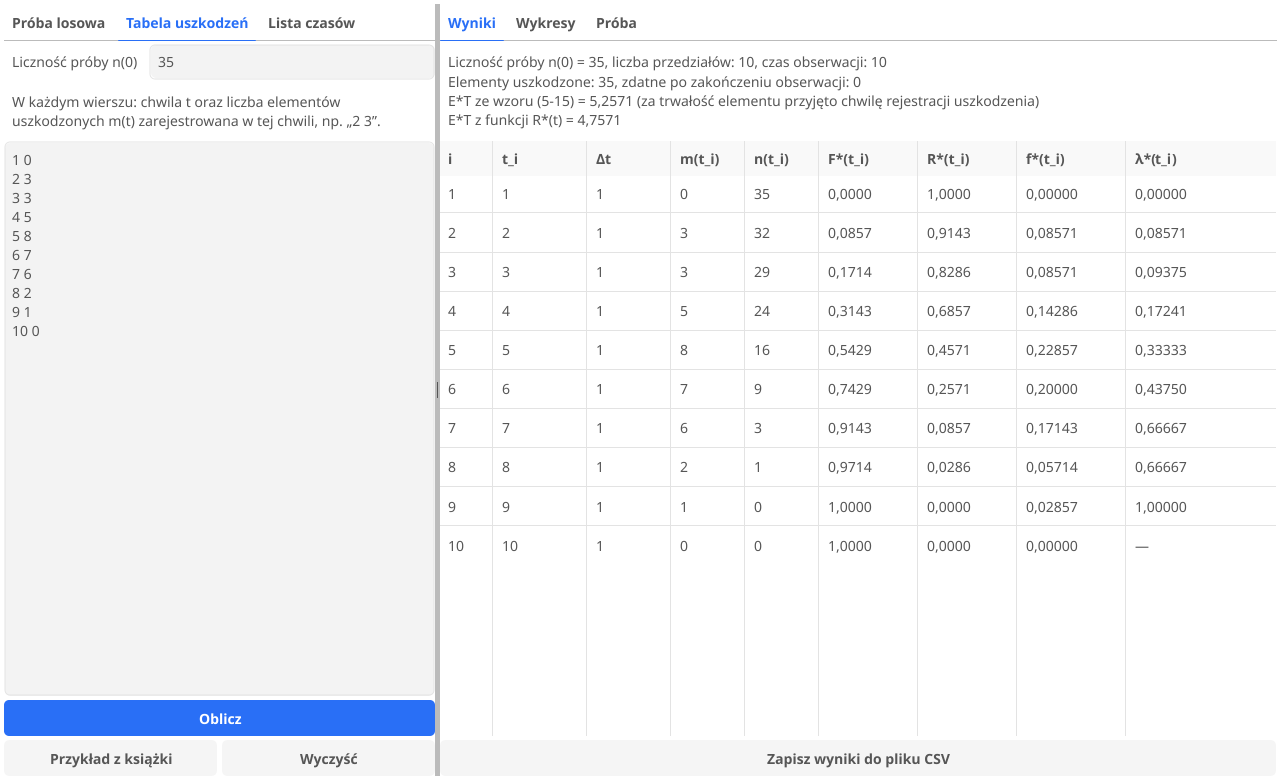
\includegraphics[width=\textwidth]{02_table_results}
  \caption{Wyniki programu dla danych z~przykładu 5.1}
  \label{fig:book-results}
\end{figure}

\begin{figure}[H]
  \centering
  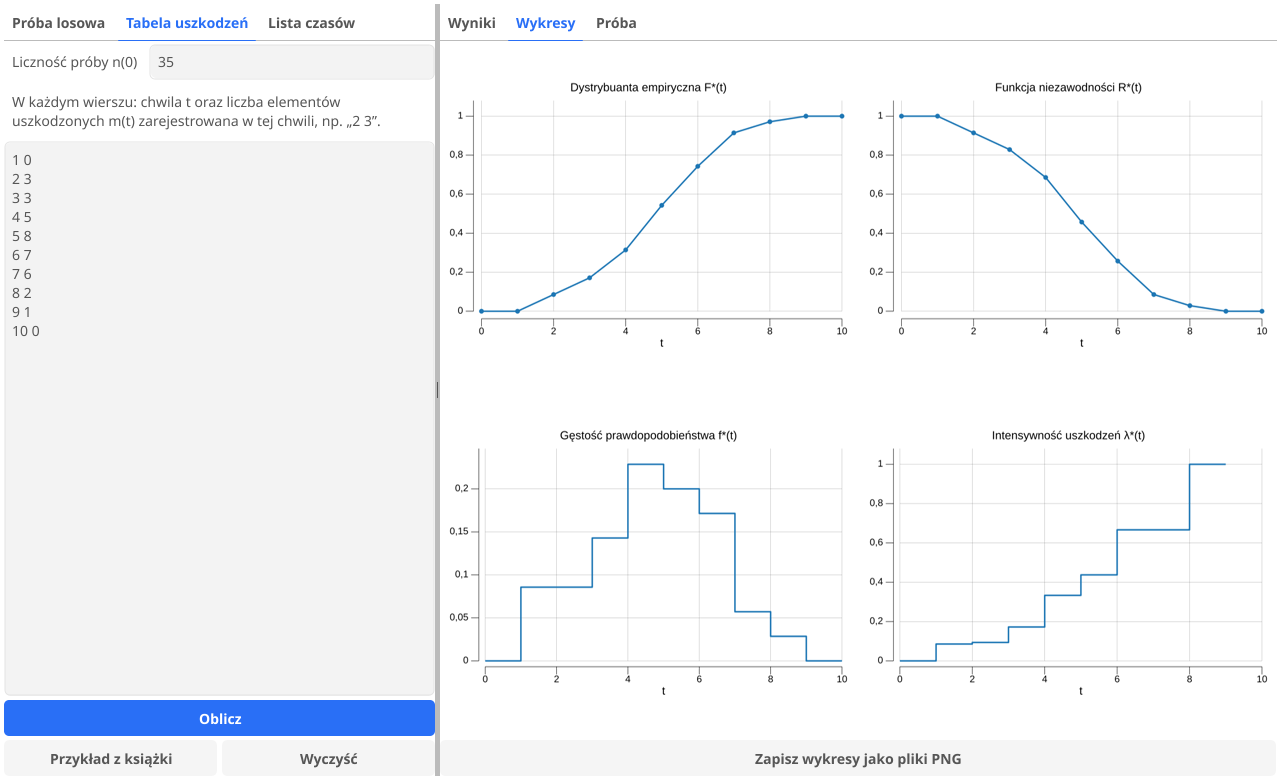
\includegraphics[width=\textwidth]{03_table_charts}
  \caption{Wykresy wskaźników dla danych z~przykładu 5.1}
  \label{fig:book-charts}
\end{figure}

\subsection{Próba losowa a~rozkład teoretyczny}

Dla każdego z~trzech rozkładów wylosowano próby o~liczności 100, 1000 i~10\,000
(ziarno generatora~1, parametry domyślne, $\Delta t$ dobierane automatycznie)
i~porównano wskaźniki empiryczne z~teoretycznymi (tab.~\ref{tab:random}). Wyniki można
odtworzyć w~programie, wpisując te same ustawienia.

\begin{table}[H]
  \centering
  \caption{Wskaźniki empiryczne dla prób losowych; $\max|F^* - F|$ to największa różnica
    między dystrybuantą empiryczną i~teoretyczną w~chwilach $t_i$}
  \label{tab:random}
  \small
  \begin{tabular}{@{}lrrrrrrr@{}}
    \toprule
    Rozkład & $n$ & $\Delta t$ & $k$ & $E^*T$ (5-15) & $E^*T$ z~$R^*$ & $ET$ & $\max|F^* - F|$ \\
    \midrule
    wykładniczy & 100 & 50 & 10 & 104,82 & 103,50 & 100,00 & 0,0479 \\
    $\lambda = 0{,}01$ & 1000 & 25 & 27 & 100,57 & 101,08 & 100,00 & 0,0099 \\
    & 10\,000 & 20 & 47 & 99,00 & 99,30 & 100,00 & 0,0043 \\
    \midrule
    Weibulla & 100 & 25 & 9 & 90,94 & 89,00 & 88,62 & 0,0479 \\
    $\beta = 2$, $\eta = 100$ & 1000 & 10 & 26 & 88,93 & 88,67 & 88,62 & 0,0099 \\
    & 10\,000 & 10 & 31 & 88,26 & 88,22 & 88,62 & 0,0049 \\
    \midrule
    normalny & 100 & 20 & 7 & 101,30 & 100,40 & 100,00 & 0,0513 \\
    $\mu = 100$, $\sigma = 20$ & 1000 & 10 & 17 & 100,23 & 100,22 & 100,00 & 0,0125 \\
    & 10\,000 & 5 & 37 & 99,71 & 99,73 & 100,00 & 0,0074 \\
    \bottomrule
  \end{tabular}
\end{table}

Wraz ze wzrostem liczności próby wskaźniki empiryczne zbliżają się do teoretycznych:
największa różnica dystrybuant maleje z~około $0{,}05$ dla $n = 100$ do poniżej
$0{,}01$ dla $n = 10\,000$, a~błąd względny $E^*T$ -- z~kilku procent do najwyżej
jednego procenta. Wykresy (rys.~\ref{fig:exponential}--\ref{fig:normal}) pokazują
zgodność przebiegów empirycznych (linia ciągła) z~teoretycznymi (linia przerywana).
Kształt $\lambda^*(t)$ odpowiada teorii: intensywność jest stała dla rozkładu
wykładniczego i~rośnie dla rozkładów Weibulla ($\beta = 2$) i~normalnego. Na końcu
osi czasu przebieg $\lambda^*$ staje się nieregularny, ponieważ zostaje już tylko
kilka zdatnych elementów i~pojedyncze uszkodzenie silnie zmienia wynik.

\begin{figure}[H]
  \centering
  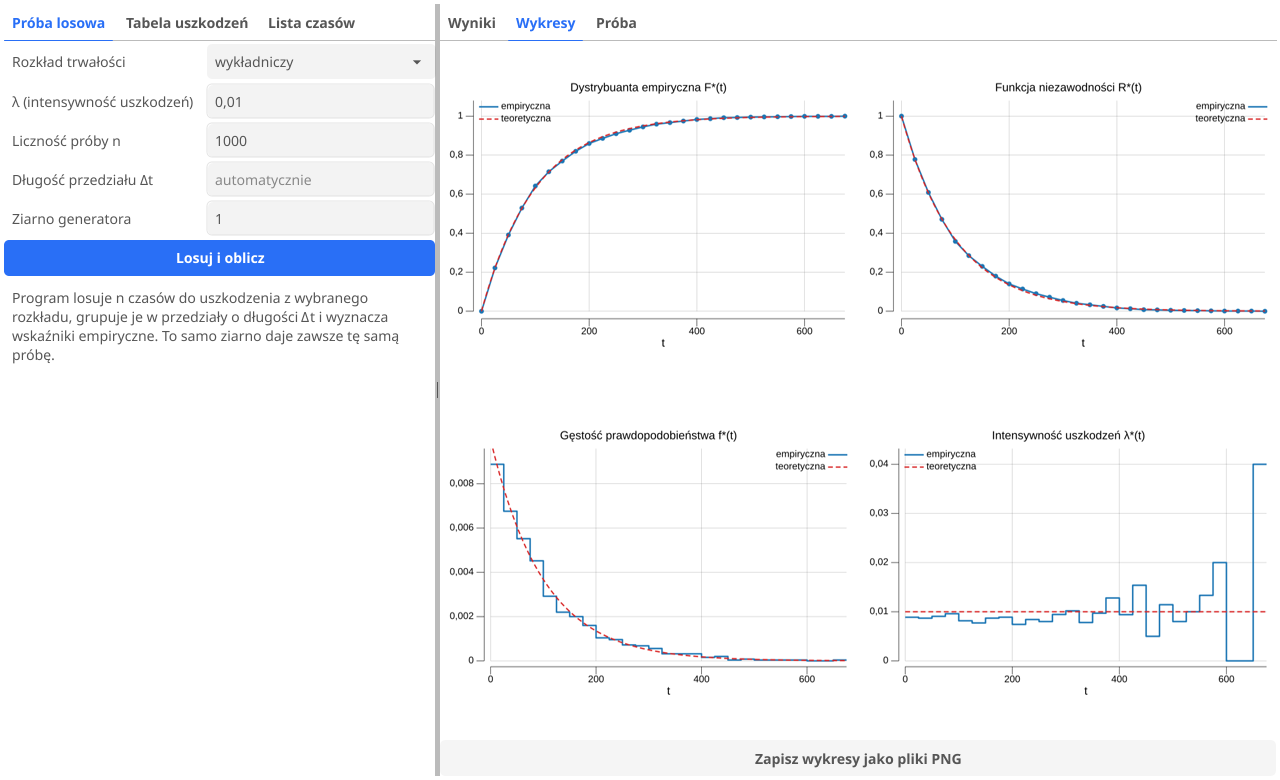
\includegraphics[width=\textwidth]{07_random_exponential_charts}
  \caption{Próba losowa z~rozkładu wykładniczego, $n = 1000$, ziarno 1}
  \label{fig:exponential}
\end{figure}

\begin{figure}[H]
  \centering
  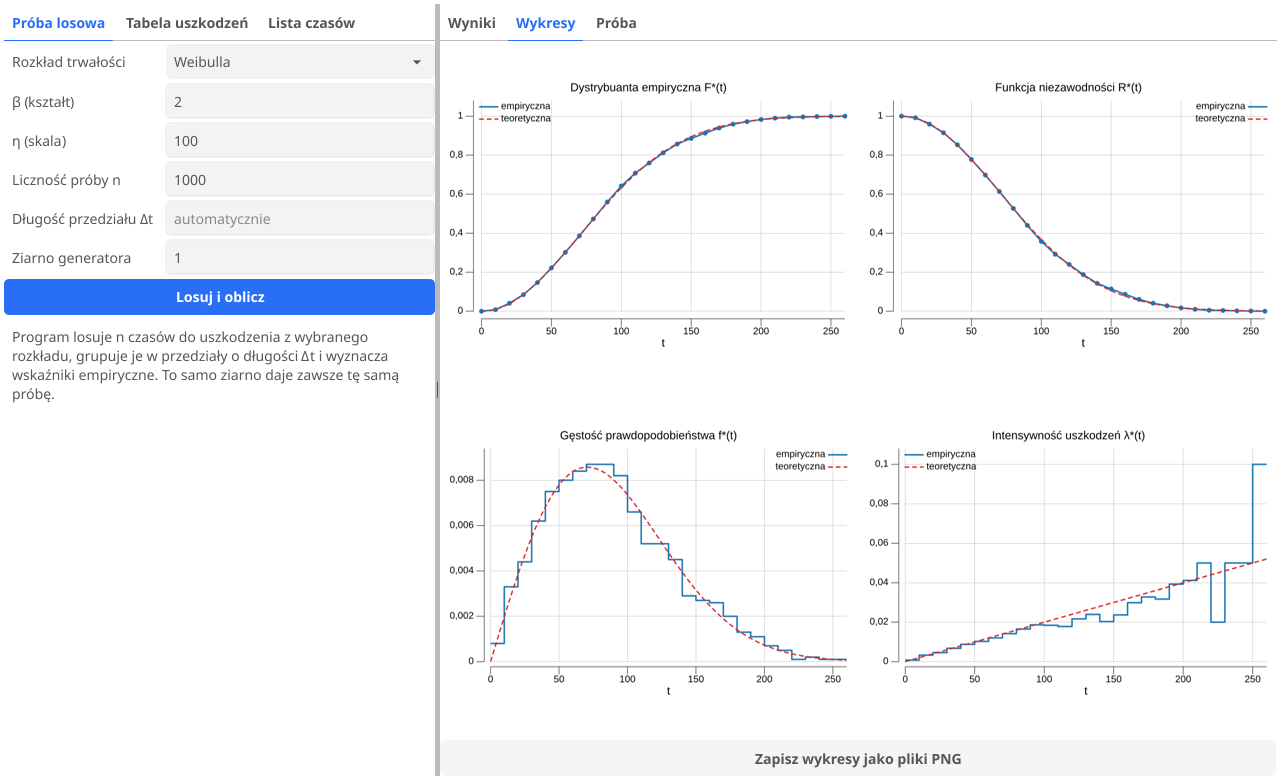
\includegraphics[width=\textwidth]{07_random_weibull_charts}
  \caption{Próba losowa z~rozkładu Weibulla, $n = 1000$, ziarno 1}
  \label{fig:weibull}
\end{figure}

\begin{figure}[H]
  \centering
  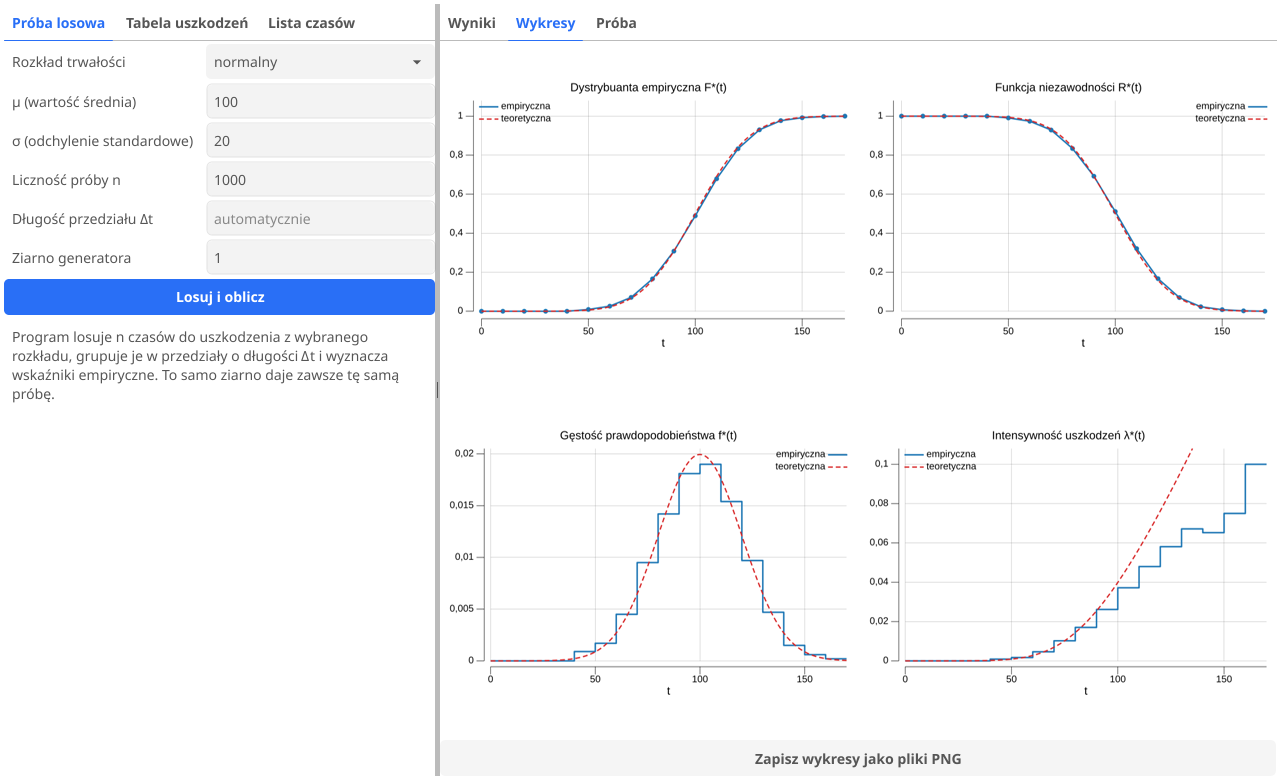
\includegraphics[width=\textwidth]{07_random_normal_charts}
  \caption{Próba losowa z~rozkładu normalnego, $n = 1000$, ziarno 1}
  \label{fig:normal}
\end{figure}

\subsection{Wpływ długości przedziału na wyniki}

Na rys.~\ref{fig:exponential} empiryczna intensywność uszkodzeń leży nieco poniżej
teoretycznej. Nie jest to błąd programu, lecz cecha wzoru (5-12): odnosi on
uszkodzenia z~całego przedziału do liczby elementów zdatnych na jego początku,
podczas gdy w~trakcie przedziału elementów zdatnych ubywa. Dla rozkładu wykładniczego
udział elementów uszkodzonych w~przedziale wynosi średnio $1 - e^{-\lambda \Delta t}$,
więc wzór (5-12) daje przeciętnie
\begin{equation*}
  \lambda^* \approx \frac{1 - e^{-\lambda \Delta t}}{\Delta t} < \lambda.
\end{equation*}
Sprawdzono to dla próby z~rozkładu wykładniczego ($\lambda = 0{,}01$, $n = 10\,000$,
ziarno~1), zmieniając tylko długość przedziału (tab.~\ref{tab:step}).

\begin{table}[H]
  \centering
  \caption{Wpływ długości przedziału $\Delta t$ na wyniki; rozkład wykładniczy,
    $\lambda = 0{,}01$, $ET = 100$}
  \label{tab:step}
  \small
  \begin{tabular}{@{}rccccc@{}}
    \toprule
    $\Delta t$ & $\lambda^*(t_1)$ & $\lambda^*(t_2)$ & $\lambda^*(t_3)$
      & $\dfrac{1 - e^{-\lambda\Delta t}}{\Delta t}$ & $E^*T$ z~$R^*$ \\
    \midrule
    100 & 0,00635 & 0,00636 & 0,00640 & 0,00632 & 107,15 \\
    50 & 0,00795 & 0,00787 & 0,00788 & 0,00787 & 101,01 \\
    25 & 0,00885 & 0,00906 & 0,00880 & 0,00885 & 99,50 \\
    10 & 0,00942 & 0,00966 & 0,00951 & 0,00952 & 99,09 \\
    5 & 0,00984 & 0,00947 & 0,00991 & 0,00975 & 99,00 \\
    \bottomrule
  \end{tabular}
\end{table}

Wartości wyznaczone przez program zgadzają się z~przewidywanymi. Dla $\Delta t = 100$
intensywność jest zaniżona o~blisko 37\%, a~dla $\Delta t = 5$ -- o~około 2,5\%.
Podobnie zachowuje się $E^*T$ wyznaczana z~$R^*(t)$: przy grubych przedziałach metoda
trapezów zawyża pole pod wypukłą krzywą, a~wraz ze zmniejszaniem $\Delta t$ wynik
zbliża się do wartości $98{,}9976$ otrzymanej ze wzoru (5-15), która od $\Delta t$
nie zależy. Przedział nie może być jednak dowolnie krótki: gdy w~przedziale jest
niewiele uszkodzeń, wartości $f^*$ i~$\lambda^*$ stają się przypadkowe. Dlatego
program domyślnie dobiera około $\sqrt{n}$ przedziałów.

\subsection{Próba niepełna}

Sprawdzono przypadek, w~którym badanie zakończono przed uszkodzeniem wszystkich
elementów. W~zakładce ,,Lista czasów'' podano $n(0) = 12$, $\Delta t = 10$ oraz dziesięć
czasów uszkodzeń: 12,5; 30; 41,2; 55; 60; 61; 70; 85; 90; 120 (rys.~\ref{fig:times}).

\begin{figure}[H]
  \centering
  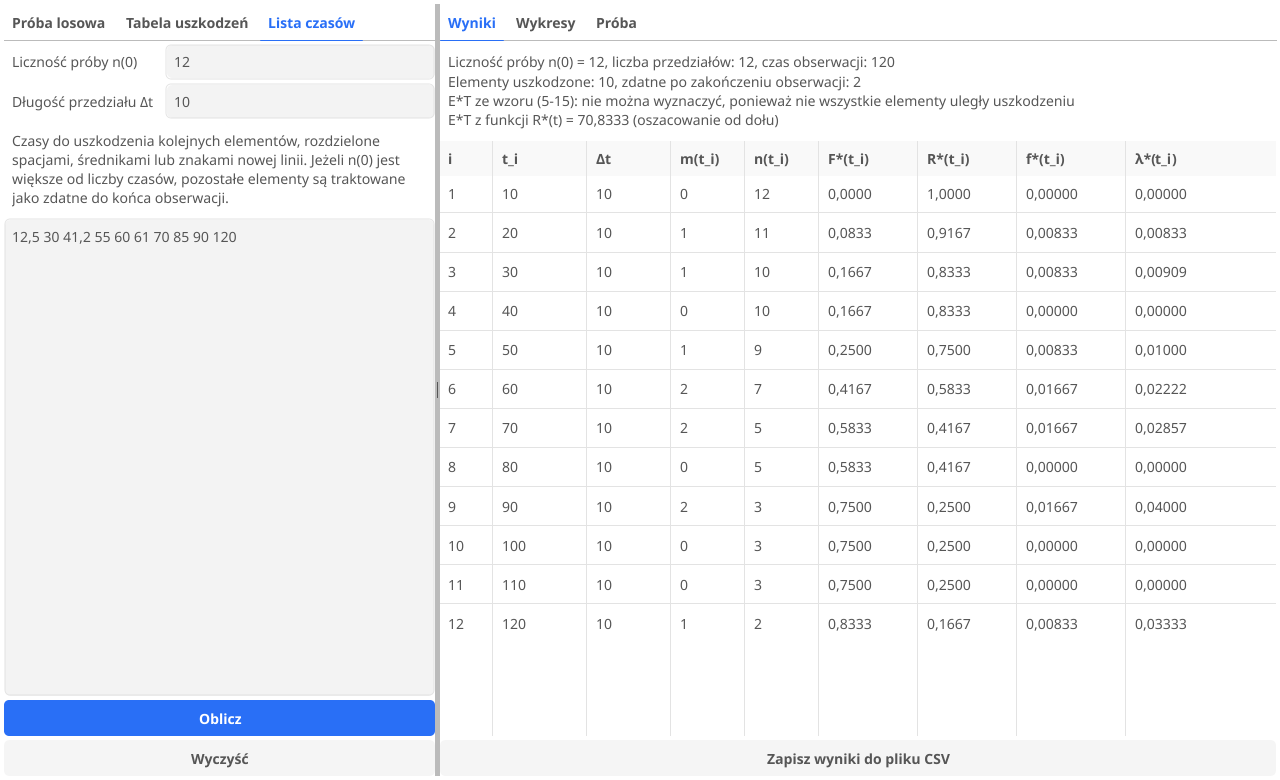
\includegraphics[width=\textwidth]{08_times_results}
  \caption{Wyniki dla listy czasów przy niepełnej próbie}
  \label{fig:times}
\end{figure}

Wyniki sprawdzono rachunkiem ręcznym. Przykładowo do przedziału $(50, 60]$ należą
czasy 55 i~60 (czas leżący na granicy trafia do niższego przedziału), a~na jego
początku zdatnych jest 9~elementów, zatem
\begin{equation*}
  F^*(60) = \frac{5}{12} = 0{,}4167, \qquad
  f^*(60) = \frac{2}{12 \cdot 10} = 0{,}01667, \qquad
  \lambda^*(60) = \frac{2}{9 \cdot 10} = 0{,}02222,
\end{equation*}
co zgadza się z~szóstym wierszem tabeli. Dwa elementy pozostały zdatne, więc
$R^*(120) = 2/12 = 0{,}1667$. Program poprawnie informuje, że $E^*T$ ze wzoru (5-15)
nie da się wyznaczyć, i~podaje oszacowanie od dołu $70{,}83$ z~całkowania $R^*(t)$.

\subsection{Obsługa błędnych danych}

Program nie wykonuje obliczeń dla błędnych danych, tylko wyświetla okno z~opisem
błędu (rys.~\ref{fig:error}), a~poprzednie wyniki pozostają bez zmian. Sprawdzone
przypadki zestawiono w~tab.~\ref{tab:errors}.

\begin{table}[H]
  \centering
  \caption{Reakcja programu na błędne dane}
  \label{tab:errors}
  \small
  \begin{tabular}{@{}p{0.36\textwidth}p{0.6\textwidth}@{}}
    \toprule
    Wprowadzone dane & Komunikat \\
    \midrule
    pusta tabela uszkodzeń & tabela uszkodzeń jest pusta \\
    $n(0)$ = ,,abc'' & Liczność próby n(0): ,,abc'' nie jest poprawną liczbą całkowitą \\
    tabela z~przykładu 5.1 przy $n(0) = 10$ & pozycja 4: łączna liczba uszkodzeń przekracza
      liczność próby n(0) \\
    wiersz tabeli z~jedną wartością & wiersz 2: oczekiwano dwóch wartości: t oraz m(t) \\
    parametr $\lambda = -1$ & parametr $\lambda$ musi być dodatni \\
    ziarno generatora ,,x'' & Ziarno generatora: ,,x'' nie jest nieujemną liczbą całkowitą \\
    liczność próby losowej $n = 0$ & liczność próby musi być liczbą dodatnią \\
    $\Delta t = 0$ & długość przedziału $\Delta t$ musi być dodatnia \\
    lista czasów ,,1 x 3'' & pozycja 2: ,,x'' nie jest poprawną liczbą \\
    trzy czasy przy $n(0) = 2$ & liczność próby n(0) jest mniejsza od liczby podanych czasów \\
    \bottomrule
  \end{tabular}
\end{table}

\begin{figure}[H]
  \centering
  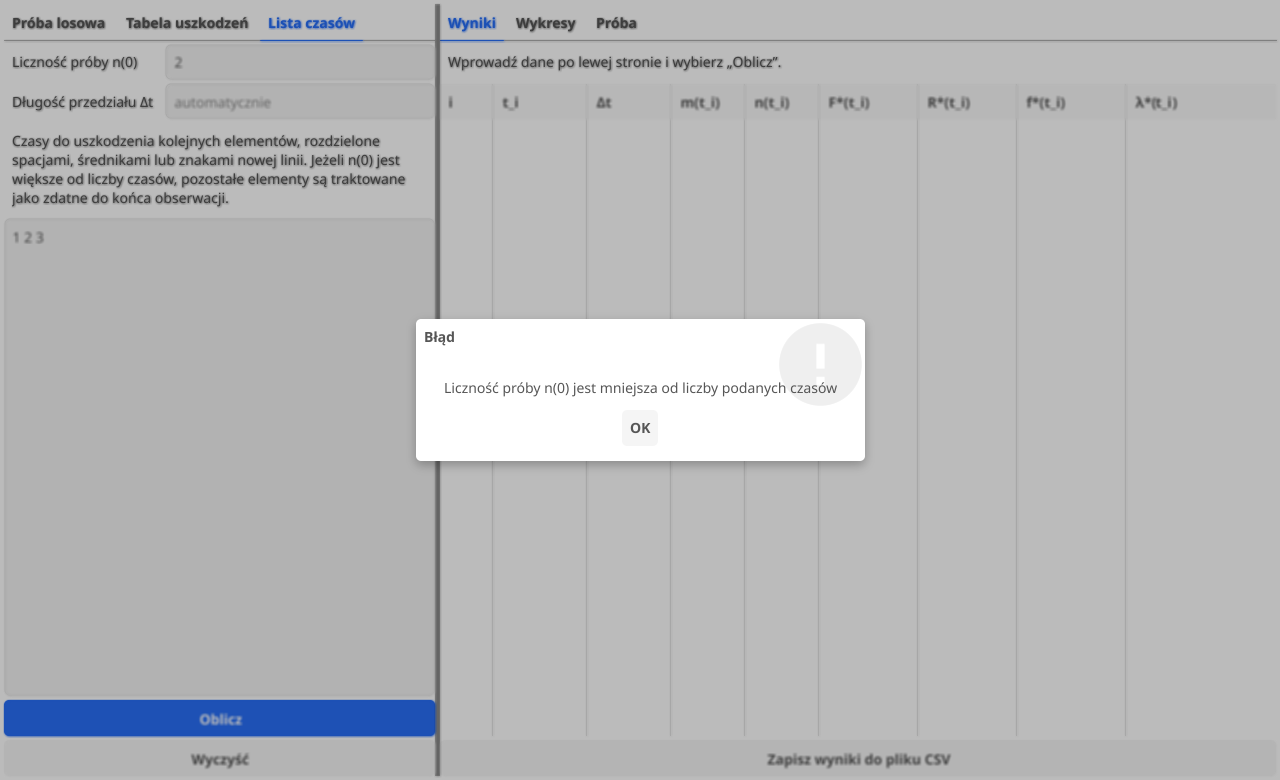
\includegraphics[width=0.78\textwidth]{09_error_dialog}
  \caption{Komunikat o~błędnych danych}
  \label{fig:error}
\end{figure}

\subsection{Wnioski}

\begin{itemize}
  \item Program odtwarza wyniki przykładów 5.1--5.4 z~książki z~dokładnością do
    zaokrągleń w~niej zastosowanych.
  \item Dla prób losowych wskaźniki empiryczne zbliżają się do teoretycznych wraz ze
    wzrostem liczności próby, zgodnie z~oczekiwaniami.
  \item Empiryczna intensywność uszkodzeń wyznaczana ze wzoru (5-12) jest zaniżona
    tym bardziej, im dłuższy jest przedział $\Delta t$; długość przedziału trzeba
    więc dobierać jako kompromis między tym błędem a~rozrzutem wyników.
  \item Błędne dane są wykrywane przed obliczeniami i~opisywane komunikatem
    wskazującym miejsce błędu.
\end{itemize}

\clearpage
\section{Instrukcja obsługi programu}

\subsection{Uruchomienie}

Program jest jednym plikiem wykonywalnym \code{empirical-reliability.exe} (Windows 10/11,
64 bity). Nie wymaga instalacji ani dodatkowych plików -- wystarczy go uruchomić.
Do działania potrzebny jest sterownik karty graficznej z~obsługą OpenGL, dostępny
standardowo w~systemie. Wersję dla systemu Linux lub macOS buduje się z~kodu
źródłowego (p.~\ref{sec:build}).

\subsection{Okno programu}

Okno jest podzielone na dwie części (rys.~\ref{fig:start}). Po lewej stronie
wprowadza się dane w~jednej z~trzech zakładek: ,,Próba losowa'', ,,Tabela uszkodzeń''
albo ,,Lista czasów''. Po prawej stronie znajdują się wyniki w~zakładkach ,,Wyniki'',
,,Wykresy'' i~,,Próba''. Granicę między częściami można przesuwać myszą.

Liczby można wpisywać z~przecinkiem albo z~kropką dziesiętną (np. \code{0,01} lub
\code{0.01}). Każde obliczenie zastępuje poprzednie wyniki.

\begin{figure}[H]
  \centering
  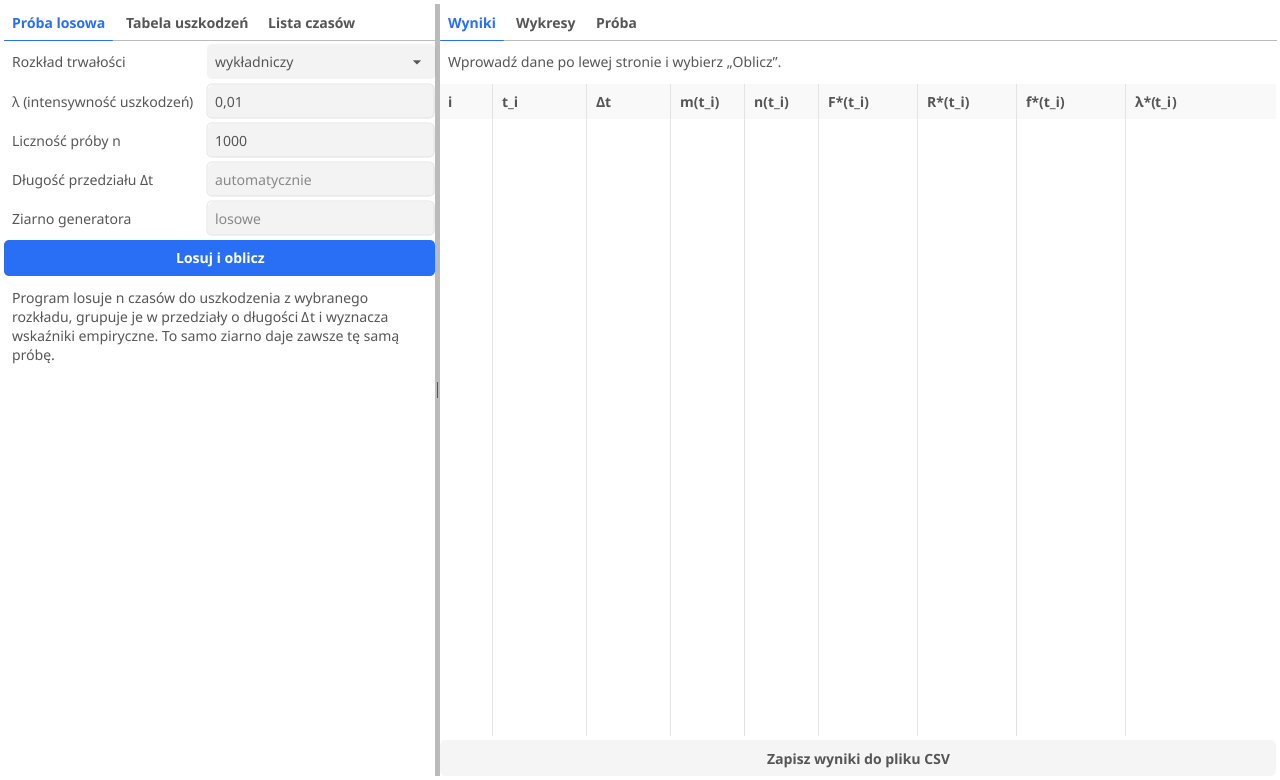
\includegraphics[width=\textwidth]{01_start}
  \caption{Okno programu po uruchomieniu}
  \label{fig:start}
\end{figure}

\subsection{Próba losowa}

Zakładka służy do wylosowania czasów do uszkodzenia z~rozkładu teoretycznego.
\begin{enumerate}
  \item Wybrać \textbf{rozkład trwałości}: wykładniczy, Weibulla albo normalny.
  \item Podać \textbf{parametry rozkładu} -- pola zmieniają się zależnie od rozkładu
    i~są wypełnione wartościami domyślnymi: $\lambda$ dla wykładniczego; $\beta$
    (kształt) i~$\eta$ (skala) dla Weibulla; $\mu$ i~$\sigma$ dla normalnego.
    Wszystkie parametry muszą być dodatnie.
  \item Podać \textbf{liczność próby $n$} (od 1 do 1\,000\,000).
  \item Opcjonalnie podać \textbf{długość przedziału $\Delta t$}. Puste pole oznacza
    dobór automatyczny.
  \item Opcjonalnie podać \textbf{ziarno generatora} (nieujemna liczba całkowita).
    To samo ziarno daje zawsze tę samą próbę; przy pustym polu każde losowanie jest
    inne, a~użyte ziarno jest pokazywane w~podsumowaniu wyników.
  \item Nacisnąć \textbf{,,Losuj i~oblicz''}.
\end{enumerate}

\subsection{Tabela uszkodzeń}

Zakładka służy do wprowadzenia danych pogrupowanych, takich jak w~przykładach
z~książki.
\begin{enumerate}
  \item Podać \textbf{liczność próby $n(0)$}.
  \item W~polu tekstowym wpisać tabelę: w~każdym wierszu chwilę $t$ oraz liczbę
    elementów uszkodzonych $m(t)$ zarejestrowaną w~tej chwili, rozdzielone spacją,
    tabulatorem lub średnikiem, np. \code{2 3}. Chwile muszą być dodatnie i~rosnące,
    ale odstępy między nimi nie muszą być równe. Puste wiersze są pomijane.
  \item Nacisnąć \textbf{,,Oblicz''}.
\end{enumerate}
Suma uszkodzeń może być mniejsza od $n(0)$ -- pozostałe elementy są wtedy traktowane
jako zdatne po zakończeniu obserwacji. Przycisk ,,Przykład z~książki'' wczytuje dane
z~przykładu 5.1, a~,,Wyczyść'' usuwa zawartość formularza.

\subsection{Lista czasów}

Zakładka służy do wprowadzenia pojedynczych czasów uszkodzeń.
\begin{enumerate}
  \item W~polu tekstowym wpisać czasy do uszkodzenia kolejnych elementów, rozdzielone
    spacjami, średnikami lub znakami nowej linii, w~dowolnej kolejności.
  \item Opcjonalnie podać \textbf{liczność próby $n(0)$}. Puste pole oznacza, że
    liczność jest równa liczbie podanych czasów. Jeżeli $n(0)$ jest większe, pozostałe
    elementy są traktowane jako zdatne do końca obserwacji.
  \item Opcjonalnie podać \textbf{długość przedziału $\Delta t$}.
  \item Nacisnąć \textbf{,,Oblicz''}.
\end{enumerate}

\subsection{Wyniki}

Zakładka ,,Wyniki'' (rys.~\ref{fig:random-results}) zawiera podsumowanie i~tabelę.
W~podsumowaniu podane są: liczność próby, liczba przedziałów i~czas obserwacji,
liczba elementów uszkodzonych i~zdatnych, $E^*T$ ze wzoru (5-15) oraz $E^*T$
z~funkcji $R^*(t)$, a~dla próby losowej także rozkład, jego parametry, użyte ziarno
i~teoretyczna wartość oczekiwana $ET$. Kolumny tabeli opisano w~tab.~\ref{tab:columns}.

\begin{table}[H]
  \centering
  \caption{Kolumny tabeli wyników}
  \label{tab:columns}
  \small
  \begin{tabular}{@{}ll@{}}
    \toprule
    Kolumna & Znaczenie \\
    \midrule
    $i$ & numer przedziału \\
    $t_i$ & koniec przedziału (chwila rejestracji) \\
    $\Delta t$ & długość przedziału \\
    $m(t_i)$ & liczba elementów uszkodzonych w~przedziale \\
    $n(t_i)$ & liczba elementów zdatnych w~chwili $t_i$ \\
    $F^*(t_i)$ & dystrybuanta empiryczna \\
    $R^*(t_i)$ & empiryczna funkcja niezawodności \\
    $f^*(t_i)$ & empiryczna gęstość prawdopodobieństwa \\
    $\lambda^*(t_i)$ & empiryczna intensywność uszkodzeń \\
    \bottomrule
  \end{tabular}
\end{table}

Znak ,,---'' w~kolumnie $\lambda^*(t_i)$ oznacza wartość nieokreśloną: na początku
przedziału nie było już elementów zdatnych. Jeżeli nie wszystkie elementy uległy
uszkodzeniu, $E^*T$ ze wzoru (5-15) nie jest wyznaczana, a~wartość z~funkcji $R^*(t)$
jest oszacowaniem od dołu.

\begin{figure}[H]
  \centering
  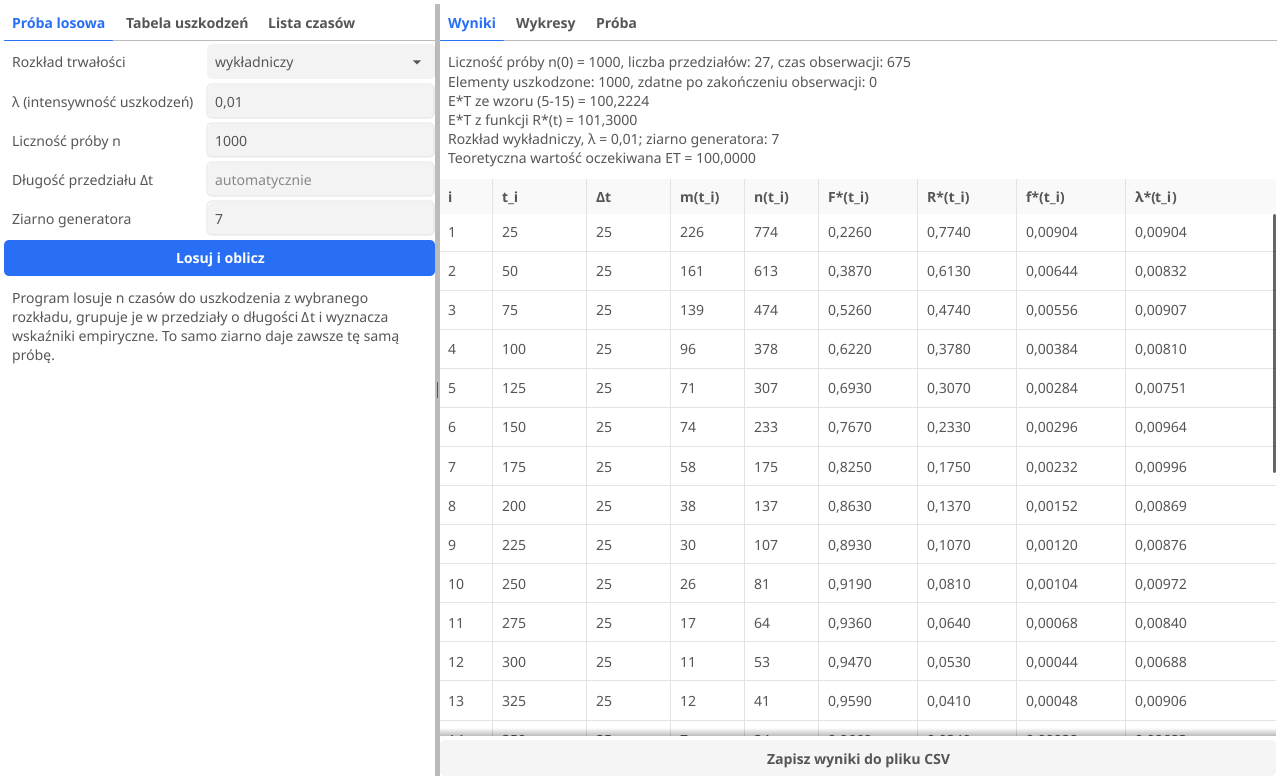
\includegraphics[width=\textwidth]{04_random_results}
  \caption{Zakładka ,,Wyniki'' dla próby losowej}
  \label{fig:random-results}
\end{figure}

\subsection{Wykresy}

Zakładka ,,Wykresy'' (rys.~\ref{fig:random-charts}) pokazuje przebiegi $F^*(t)$,
$R^*(t)$, $f^*(t)$ i~$\lambda^*(t)$. Dystrybuanta i~funkcja niezawodności są
narysowane jako punkty w~chwilach $t_i$ połączone odcinkami. Gęstość i~intensywność
uszkodzeń dotyczą całych przedziałów, dlatego są narysowane jako wykresy schodkowe.
Dla próby losowej czerwona linia przerywana pokazuje przebieg teoretyczny rozkładu,
z~którego losowano.

\begin{figure}[H]
  \centering
  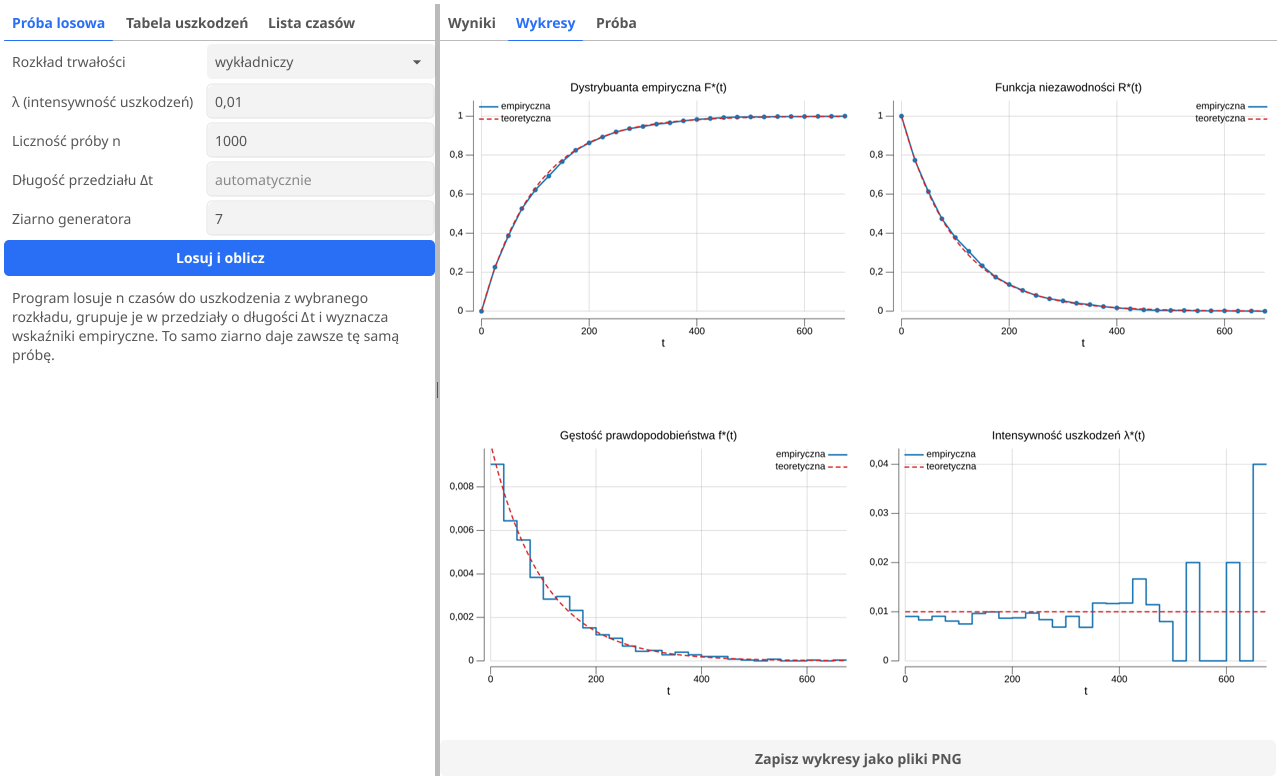
\includegraphics[width=\textwidth]{05_random_charts}
  \caption{Zakładka ,,Wykresy'' dla próby losowej}
  \label{fig:random-charts}
\end{figure}

\subsection{Próba}

Zakładka ,,Próba'' (rys.~\ref{fig:random-sample}) zawiera pojedyncze czasy uszkodzeń
posortowane rosnąco -- wylosowane albo wpisane w~zakładce ,,Lista czasów''. Można je
zaznaczyć i~skopiować, na przykład po to, by wkleić je do zakładki ,,Lista czasów''
i~przeliczyć z~inną długością przedziału. Dla danych z~tabeli uszkodzeń zakładka jest
pusta, ponieważ pojedyncze czasy nie są wtedy znane.

\begin{figure}[H]
  \centering
  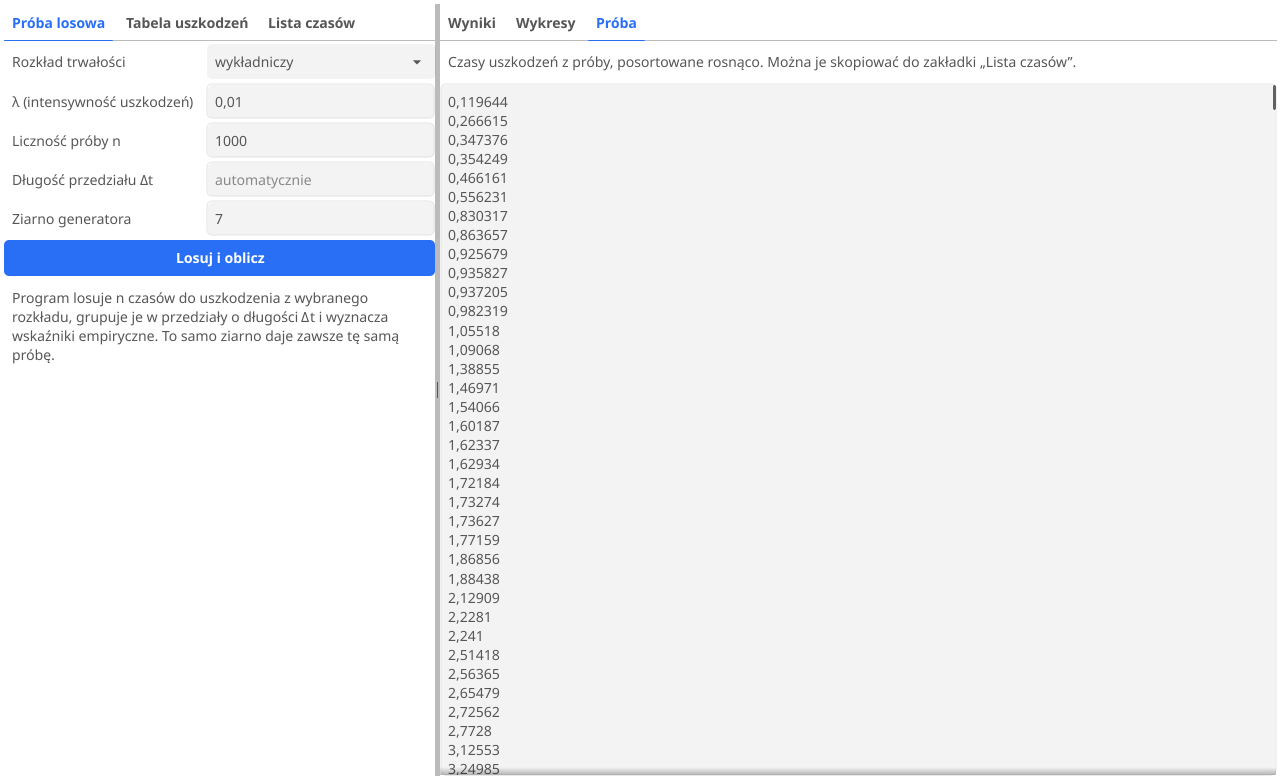
\includegraphics[width=\textwidth]{06_random_sample}
  \caption{Zakładka ,,Próba'' z~wylosowanymi czasami}
  \label{fig:random-sample}
\end{figure}

\subsection{Zapis wyników}

\begin{itemize}
  \item \textbf{,,Zapisz wyniki do pliku CSV''} (zakładka ,,Wyniki'') zapisuje tabelę
    wyników oraz wartości $n(0)$ i~$E^*T$. Plik ma domyślną nazwę \code{results.csv},
    średnik jako separator kolumn i~przecinek dziesiętny, więc otwiera się
    bezpośrednio w~polskiej wersji programu Excel.
  \item \textbf{,,Zapisz wykresy jako pliki PNG''} (zakładka ,,Wykresy'') zapisuje
    cztery wykresy do wskazanego folderu jako \code{cdf.png} (dystrybuanta),
    \code{reliability.png} (funkcja niezawodności), \code{density.png} (gęstość)
    i~\code{hazard.png} (intensywność uszkodzeń).
\end{itemize}
Oba przyciski działają dopiero po wykonaniu obliczeń.

\subsection{Komunikaty o~błędach}

Jeżeli dane są niepoprawne, program wyświetla okno z~opisem błędu (rys.~\ref{fig:error})
i~nie zmienia wyników. Komunikat wskazuje pole formularza, numer wiersza tabeli albo
pozycję na liście czasów, w~której wykryto błąd. Po zamknięciu okna przyciskiem
,,OK'' należy poprawić dane i~ponowić obliczenia. Przykłady komunikatów zawiera
tab.~\ref{tab:errors}.

\subsection{Budowanie programu z~kodu źródłowego}
\label{sec:build}

Do zbudowania programu potrzebne są: Go w~wersji 1.26 lub nowszej oraz kompilator
języka C, którego wymaga biblioteka Fyne. Plik wykonywalny buduje się na tym
systemie, na którym ma działać, poleceniem wydanym w~katalogu głównym programu
(tab.~\ref{tab:build}). Wynikiem jest zawsze jeden plik wykonywalny.

\begin{table}[H]
  \centering
  \caption{Budowanie programu w~poszczególnych systemach}
  \label{tab:build}
  \small
  \begin{tabular}{@{}l>{\raggedright\arraybackslash}p{0.3\textwidth}>{\raggedright\arraybackslash}p{0.48\textwidth}@{}}
    \toprule
    System & Dodatkowe wymagania & Polecenie \\
    \midrule
    Windows & gcc (MinGW-w64) &
      \code{go build -ldflags "-H=windowsgui -s -w" -o empirical-reliability.exe .} \\
    Linux & pakiety \code{gcc}, \code{libgl1-mesa-dev}, \code{xorg-dev}, \code{libxkbcommon-dev}, \code{libwayland-dev} &
      \code{go build -ldflags "-s -w" -o empirical-reliability .} \\
    macOS & narzędzia wiersza poleceń Xcode &
      \code{go build -ldflags "-s -w" -o empirical-reliability .} \\
    \bottomrule
  \end{tabular}
\end{table}


\begin{thebibliography}{9}
  \bibitem{prazewska}
    \emph{Niezawodność urządzeń elektronicznych}. Praca zbiorowa pod red. M.~Prażewskiej.
    Wydawnictwa Komunikacji i~Łączności, Warszawa 1987, s.~208--213.
  \bibitem{go}
    \emph{The Go Programming Language}. Dokumentacja języka i~biblioteki standardowej,
    \url{https://go.dev/doc/}.
  \bibitem{fyne}
    \emph{Fyne}. Biblioteka graficznego interfejsu użytkownika dla języka Go,
    \url{https://fyne.io}.
  \bibitem{gonum}
    \emph{Gonum Plot}. Biblioteka do rysowania wykresów dla języka Go,
    \url{https://github.com/gonum/plot}.
\end{thebibliography}

\end{document}
